% CAP description for Tree --> Expand by Indexpath --> Indexpath

Use this parameter to specify the indexpath of the subtree you want to expand.   Make sure you give the whole path (either starting from the top of the tree, or at the position defined by the pre-ascend and path type parameters).

\begin{itemize}
\item Enter the path to the item as an indexpath.
\item Use slash {\tt '/'} as a path separator (to separate parent nodes from child nodes).
\item For example, \bxshell{1/2} (without quotes). 
\bxtipp{The first node is '1' (without quotes)}

  \end{itemize}



\textbf{Example:}

\begin{itemize}
\item Your tree looks like this:

\begin{figure}
\begin{center}
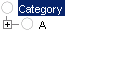
\includegraphics{PS/Treeexample3}
\caption{Tree 3}
\label{treeexample3}
\end{center}
\end{figure}

\item You want to expand the tree to node A
\item Enter \bxshell{1/1}:

\begin{figure}
\begin{center}
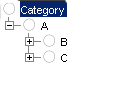
\includegraphics{PS/Treeexample4}
\caption{Tree 4}
\label{treeexample4}
\end{center}
\end{figure}
\end{itemize}
